\documentclass[12pt,a4paper]{article}
\synctex=1
\usepackage[utf8]{inputenc}
\usepackage[margin=1cm]{geometry}
\usepackage{graphicx}
%\usepackage{verbatim}
\usepackage{listings}
\usepackage{textcomp}
\usepackage{courier}
\usepackage{libertine}
\usepackage{pgfornament}
\usepackage{eso-pic}
\usepackage{amsmath}
\usepackage{amsfonts}
\usepackage{amssymb}
\usepackage[hangul]{kotex}
\linespread{1.3}

\title{
	\centering
	\pgfornament[width=12cm,color=teal]{84}\\
	\vspace{1cm}
	\fontsize{50}{50} \selectfont {File Browser\\inspired by MindMap}
		\pgfornament[width=12cm,color=teal]{88}\\
	\vfill}
\author{
	\LARGE
	\begin{tabular}{rl}
		\hline
		학번 : & 2016110056\\ 
		학과 : & 불교학부 \\
		이름 : & 박승원\\
		날짜 : & \today\\
		\hline
	\end{tabular}\vspace{2cm}
	\\
\includegraphics[width=0.5\textwidth]{logo.jpg}
	}
\date{}


\begin{document}
\maketitle
\pagenumbering{gobble}
\noindent
\lstset{language=C++, columns=flexible, tabsize=4, frame=shadowbox, showstringspaces=false, breaklines=true, upquote=true, basicstyle=\normalsize}
{\LARGE	개인 프로젝트를 따로 하기 때문에 gene sequencing은 그냥 간략하게 해서 냅니다.}	

\newpage
Learning Computer Science, I received many documents and data.
These data were to be referenced often and stored well.
But, it was very hard to remember where I put those files.
Every time I wander directories searching for the files, I felt weary.
So, I needed a way to systemically store files and show it in a orderly form.

I reminded the Mindmap. 
Mindmap was somewhat a tree data structure.
And directories are definately a tree.
So I thought I can make a mindmap-like file browser.

I already began this project from the beginning of this semester.
Even though it is not fully implemented, I am now using it and benefitting from it.
Now it is so easy to find and open a file I want to see. 
It is just one click away.
I used graph sturcture to represent those files and directories.
Because tree structure is a form of graph, I reconfigured the graph header file I made in data structure class of last semester to fit my needs.

Basic idea is to show what I want to show(among directories and files) at the place where I want to show them(in a big sketchbook).

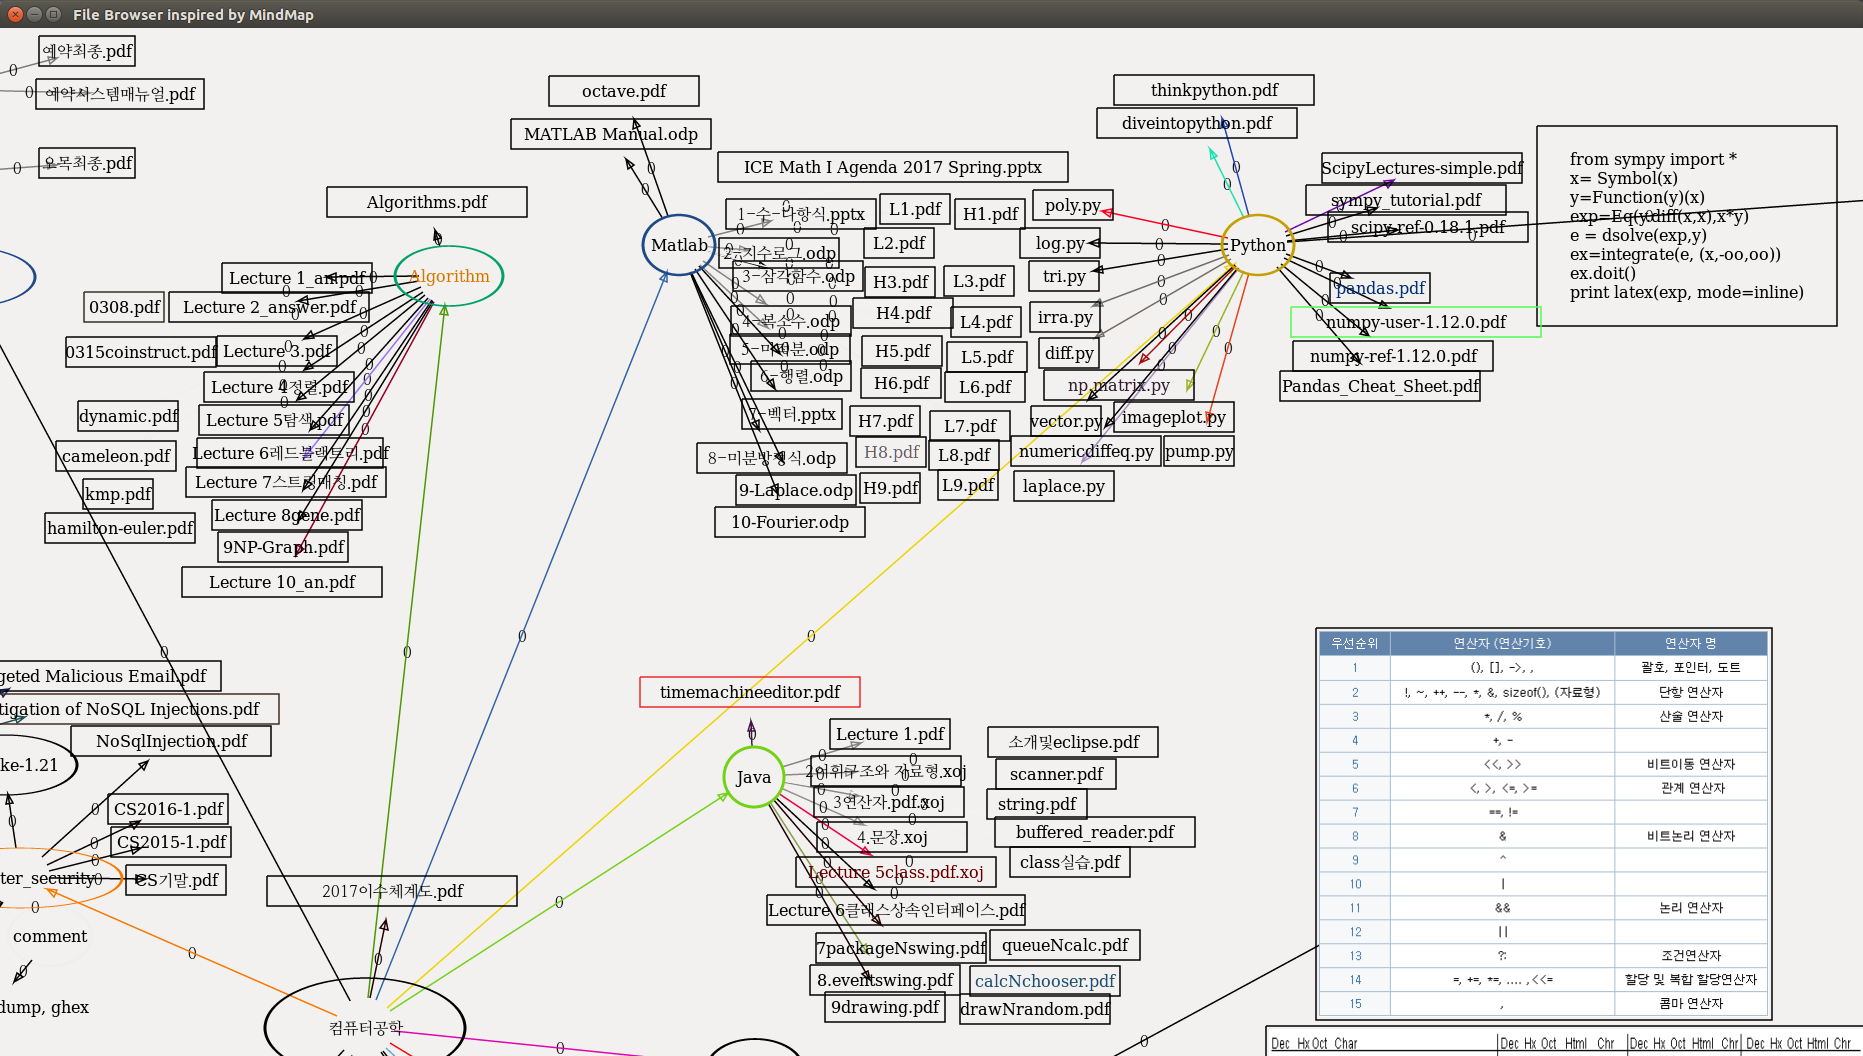
\includegraphics[width=\textwidth]{1.png}
All the characters of above picture is all file names.
But to avoid hassle of too much files, I can choose which file to show and which file to hide.
Also I can choose what type of border and arrow it will have.
One more option is to show an image files.
Now I can access hierachy of directories and files in one screen.
\newpage
If this program is polished well enough, it can alse be used as an IDE.
This is just a possibility but, I think, using mindmap like IDE is the future.
IDE is just a file browser from my point of view.

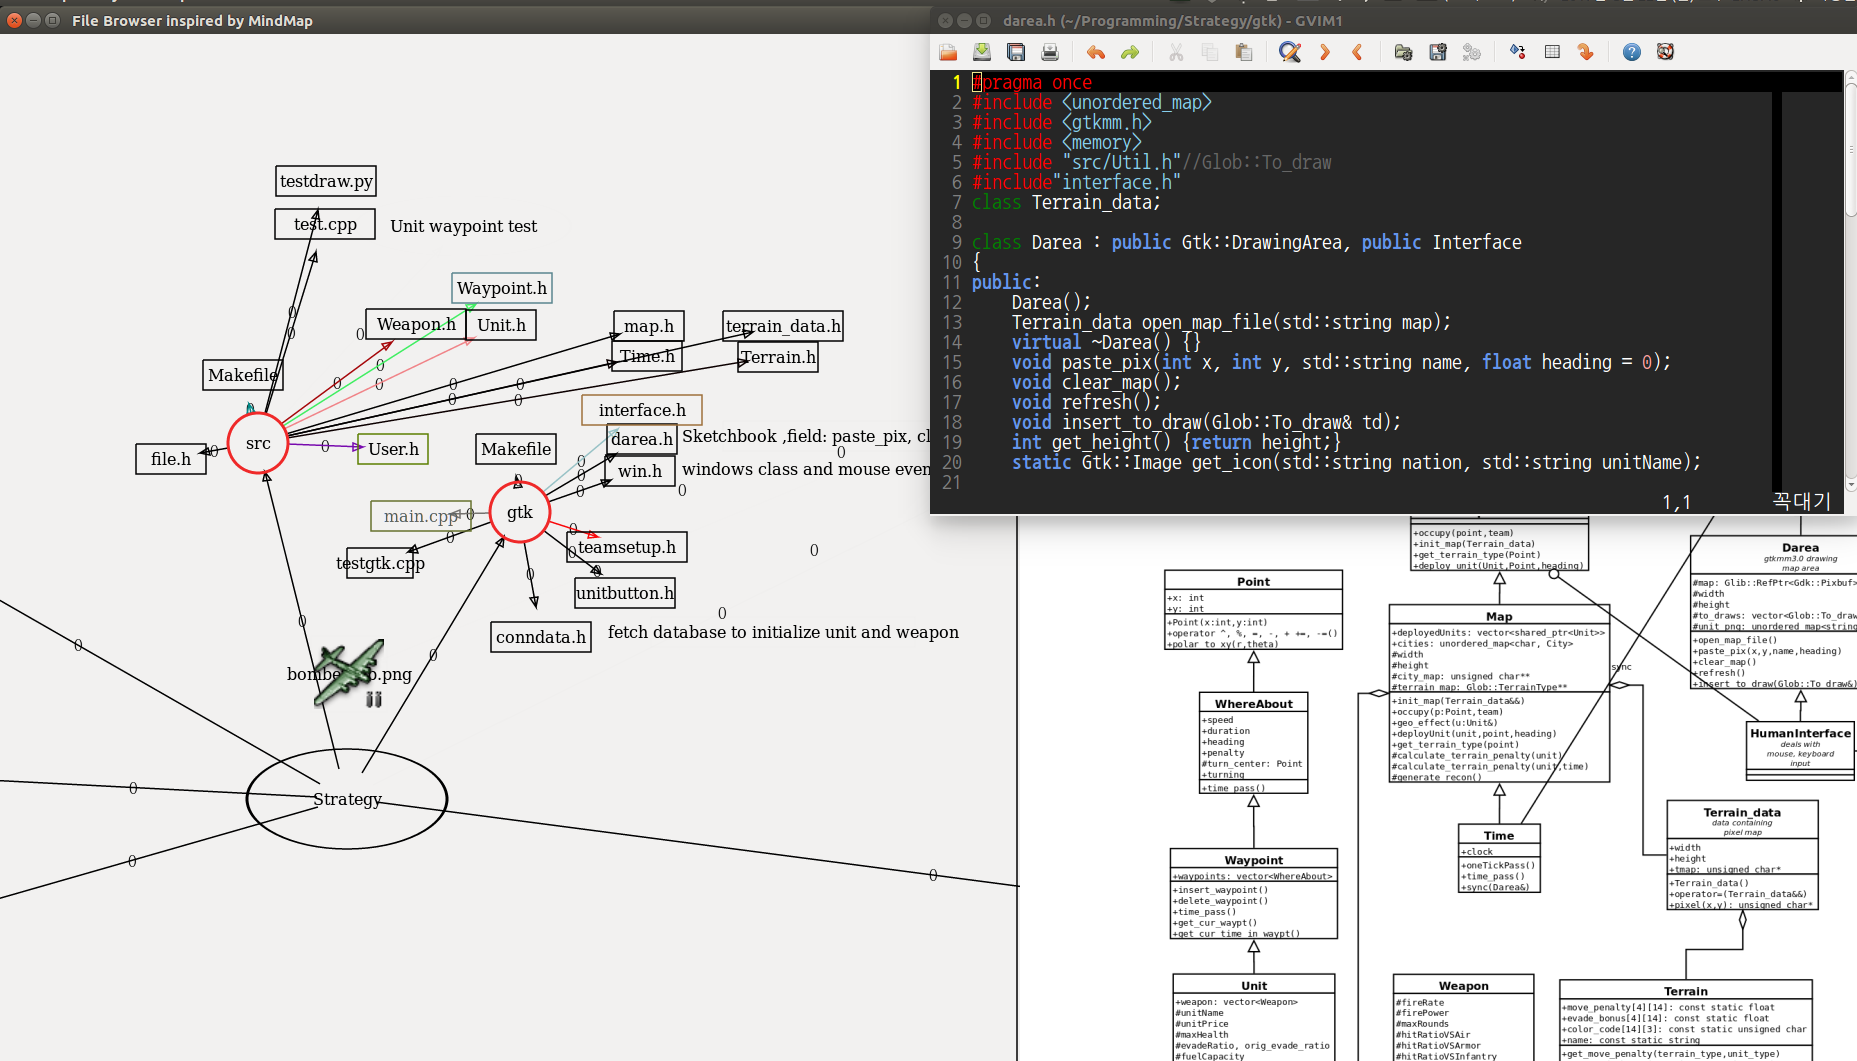
\includegraphics[width=\textwidth]{2.png}

\end{document}
